%------------------------------------------------------------------------------------------------
%
%
%      Project Name: NjustThesis Template for Bachelor of Economics , Management & Arts
%
%
%------------------------------------------------------------------------------------------------
%
%                                created by Qingyun Fang <fqy2017@gmail.com>
%
%                                             Last-modified: 2018-3-10
% 
%------------------------------------------------------------------------------------------------

\documentclass[UTF8,cs4size,a4paper,fancyhdr,twoside]{ctexbook}

\usepackage{ctex}
\usepackage[top=20mm, bottom=30mm, left=20mm, right=20mm]{geometry}   %	页边距设置
\usepackage{titlesec}              % 修改章节标题
\usepackage{fancyhdr}           % 页眉页脚
\usepackage{fancybox}          %  生成摘要页的边框
\usepackage{setspace}           % 调整行距
\usepackage{titletoc}              % 目录
\usepackage[super,square,sort & compress]{natbib}   % 参考文献设置
\usepackage[titletoc]{appendix}
\usepackage{graphicx}           %   插图
\usepackage{subfig}
\usepackage{caption}
\usepackage{listings}             %    插入代码
\usepackage[framed,numbered,autolinebreaks,useliterate]{mcode} % 插入代码
\usepackage{float}

\usepackage{tabu}                %  表格
\usepackage{booktabs}        %  表格线宏包
\usepackage{tabularx}          %  调整表格列宽
\usepackage{multirow}         %  表格合并
\usepackage{array}               %  数组宏包,用于表格宽度
\usepackage{multicol}          %  表格合并
\usepackage{longtable}        %  表格合并
\usepackage[figuresright]{rotating}   %表格合并
\usepackage{colortbl}           %  调节表格行高
\usepackage{makecell}         %   加粗表格横线

\usepackage{amsmath}        %   数学符号
\usepackage{amsthm}
\usepackage{amssymb}
\usepackage{bm}

\usepackage{url}                  %  插入网址




%------------------------------------------------------------------------------------------------
%		重新制定字体大小命令,以便后面方便使用
%------------------------------------------------------------------------------------------------

%	参考CTeX宏包说明文档中对字体大小的规定,也可以使用诸如\zihao{3}\zihao{-3}之类的命名

\newcommand{\chuhao}{\fontsize{42bp}{\baselineskip}\selectfont}
\newcommand{\xiaochu}{\fontsize{36bp}{\baselineskip}\selectfont}
\newcommand{\yihao}{\fontsize{26bp}{\baselineskip}\selectfont}
\newcommand{\xiaoyi}{\fontsize{24bp}{\baselineskip}\selectfont}
\newcommand{\erhao}{\fontsize{22bp}{\baselineskip}\selectfont}
\newcommand{\xiaoer}{\fontsize{18bp}{\baselineskip}\selectfont}
\newcommand{\sanhao}{\fontsize{16bp}{\baselineskip}\selectfont}
\newcommand{\xiaosan}{\fontsize{15bp}{\baselineskip}\selectfont}
\newcommand{\sihao}{\fontsize{14bp}{\baselineskip}\selectfont}
\newcommand{\xiaosi}{\fontsize{12bp}{\baselineskip}\selectfont}
\newcommand{\wuhao}{\fontsize{10.5bp}{\baselineskip}\selectfont}
\newcommand{\xiaowu}{\fontsize{9bp}{\baselineskip}\selectfont}


% CTeX 字体使用说明

%   \songti           宋体命令
%   \heiti              黑体命令
%   \fangsong      仿宋命令
%   \kaishu           楷书命令
%   \lishu             隶书命令
%   \youyuan       幼圆命令
%   \yahei            雅黑命令


%   XeTeX 字体使用说明

\setCJKfamilyfont{SCB}{STSongti-SC-Regular}             
\newcommand{\songtibold}{\CJKfamily{SCB}}               % 设置宋体加粗

\setCJKfamilyfont{STB}{STKaitiSC-Bold}             
\newcommand{\kaishubold}{\CJKfamily{STB}}               % 设置楷体加粗

% 中文断行
\XeTeXlinebreaklocale "zh"
\XeTeXlinebreakskip = 0pt plus 1pt minus 0.1pt

%------------------------------------------------------------------------------------------------
%		重新制定章节标题样式,包括样式和标题与上下文的间距
%------------------------------------------------------------------------------------------------

\CTEXsetup[number={\arabic{chapter}}]{chapter}
\CTEXsetup[name={,}]{chapter}
\CTEXsetup[nameformat={\heiti\xiaosan\raggedright}]{chapter}   %	Chapter章节标号格式
\CTEXsetup[titleformat={\heiti\xiaosan\raggedright}]{chapter}      %	Chapter章节标题格式
\CTEXsetup[beforeskip={-8ex}]{chapter}                          
\CTEXsetup[afterskip={1ex}]{chapter}
%\titleformat{\chapter}{\bf\heiti\xiaosan\raggedright}{\bf\heiti\arabic{chapter}}{1em}{}[]


\CTEXsetup[format={\heiti\zihao{4}\bfseries}]{section}
\CTEXsetup[format={\heiti\zihao{-4}\bfseries}]{subsection}
\CTEXsetup[format={\heiti\zihao{-4}\bfseries}]{subsubsection}

\titlespacing{\chapter}{0em}{-3ex}{1ex}
\titlespacing{\section}{0em}{0ex}{0ex}
\titlespacing{\subsection}{0em}{0ex}{0ex}
\titlespacing{\subsubsection}{0em}{0ex}{0ex}



%------------------------------------------------------------------------------------------------
%		制定页眉页脚样式、页眉高度以及页眉与正文的距离
%------------------------------------------------------------------------------------------------

%	制定页眉高度和页眉与正文的距离
\setlength{\headheight}{1.4cm}
\setlength{\headsep}{8pt}

%	制定页眉页脚样式
\fancypagestyle{plain}{
	\pagestyle{fancy}      
}

\pagestyle{fancy}
\fancyhead[C]{
	\zihao{-2}{\songtibold 本\hspace{5mm}科\hspace{5mm}毕\hspace{5mm}业\hspace{5mm}论\hspace{5mm}文}}
\fancyhead[LE,RO]{第~\thepage ~页}
\fancyhead[RE,LO]{}
\cfoot{}

\renewcommand{\headrulewidth}{0.7pt}

\makeatletter
\newcommand{\openany}{\@openrightfalse}
\newcommand{\openright}{\@openrighttrue}
\makeatother



%------------------------------------------------------------------------------------------------
%		目录格式设置
%------------------------------------------------------------------------------------------------

\renewcommand{\contentsname}{ \hspace*{\fill} 目\hspace{1.5em} 次\hspace*{\fill}}

\titlecontents{chapter}[0em]{\songti\zihao{-4}}{\thecontentslabel\ }{}
{\hspace{.5em}\titlerule*[4pt]{$\cdot$}\contentspage}
\titlecontents{section}[0em]{\vspace{0.1\baselineskip}\songti\zihao{-4}}{\thecontentslabel\ }{}
{\hspace{.5em}\titlerule*[4pt]{$\cdot$}\contentspage}
\titlecontents{subsection}[0em]{\vspace{0.1\baselineskip}\songti\zihao{-4}}{\thecontentslabel\ }{}
{\hspace{.5em}\titlerule*[4pt]{$\cdot$}\contentspage}



%------------------------------------------------------------------------------------------------
%		参考文献标题设置
%------------------------------------------------------------------------------------------------

\renewcommand\bibname{参\hspace{0.5em}考\hspace{0.5em}文\hspace{0.5em}献}



%------------------------------------------------------------------------------------------------
%		附录标题设置
%------------------------------------------------------------------------------------------------

\CTEXsetup[name={附录},number={\Alph{chapter}}]{appendix}



%------------------------------------------------------------------------------------------------
%		图片标题设置
%------------------------------------------------------------------------------------------------

\captionsetup[table]{name={表},labelsep=quad}
\captionsetup[figure]{name={图},labelsep=quad}

\DeclareCaptionFont{captionfont}{\heiti\fontsize{10.5bp}{13.65bp}\selectfont}
\captionsetup{font=captionfont}

\newcommand{\topcaption}{%
	\setlength{\abovecaptionskip}{0ex}%
	\setlength{\belowcaptionskip}{1.5ex}%
	\caption}   % 表格上标题修改


\setlength{\intextsep}{0pt}
\setlength{\textfloatsep} {0pt}



%------------------------------------------------------------------------------------------------
%		目录代码自动换行
%------------------------------------------------------------------------------------------------

\lstset{breaklines}    %自动将长的代码行换行排版
\lstset{extendedchars=false}




%------------------------------------------------------------------------------------------------
%		正文区
%------------------------------------------------------------------------------------------------
\begin{document}

\begin{titlepage}
	
	\begin{center}
		\quad\par
		\vspace{10mm}
		\begin{figure}[H]
			\centering
			
\includegraphics[width=75mm]{figure//Njust}\\
		\end{figure}
		\vspace{10mm}
		{\zihao{0}\heiti{毕业设计说明书 }}
		
		\vspace{26.5mm}
		\setlength{\extrarowheight}{7.5mm}
		\begin{tabular}{rp{8.5\ccwd}<{\centering}cp{8.\ccwd}<{\centering}}
			\zihao{3}\songtibold\textbf{\makebox[3\ccwd][s]{作\quad 者}~:}& \zihao{3}\kaishu{ 张三} & \zihao{3}\songtibold\textbf{\makebox[2.5\ccwd][s]{学\hspace{0.5em} 号}~ :}&\zihao{3}\kaishu{ 0123456789} \\
			\Xcline{2-2}{0.8pt}\Xcline{4-4}{0.8pt}
			\zihao{3}\songtibold\textbf{\makebox[3\ccwd][s]{学\quad 院}~:}&
			\multicolumn{3}{c}{\zihao{3}\kaishu{电子工程与光电技术学院}} \\
			\Xcline{2-4}{0.8pt}
			\zihao{3}\songtibold\textbf{\makebox[3\ccwd][s]{专\quad 业}~:}& \multicolumn{3}{c}{\zihao{3}\kaishu{ 通信工程}}\\
			\Xcline{2-4}{0.8pt}
			\zihao{3}\songtibold\textbf{\makebox[3\ccwd][s]{题\quad 目}~:}& \multicolumn{3}{c}{\zihao{3}\kaishu{南理工本科毕设\LaTeX 模板(理工类)设计}}\\
			\Xcline{2-4}{0.8pt}
			& \multicolumn{3}{c}{\zihao{3}\kaishu{ }}\\
			\Xcline{2-4}{0.8pt}
		\end{tabular}
		
		\vspace{20mm}
		\setlength{\extrarowheight}{0mm}
		
		\begin{tabular}{rp{10\ccwd}<{\centering}p{10\ccwd}<{\centering}}
			\sanhao\songtibold\textbf{\makebox[3\ccwd][s]{指导者}:}&\songti\sanhao\textbf{} & \songti\sanhao\textbf{}\\
			\Xcline{2-3}{0.8pt}
			\sanhao\songtibold\textbf{\makebox[3\ccwd][s]{}}&\wuhao\songti(姓\quad 名)&\wuhao\songti(专业技术职务)\\
			\rule{0pt}{8mm}& \songti\sanhao\textbf{} & \songti\sanhao\textbf{}\\
			\Xcline{2-3}{0.8pt}
			&\wuhao\songti(姓\quad 名)&\wuhao\songti(专业技术职务)\\
		\end{tabular}
		
		\begin{tabular}{rp{10\ccwd}<{\centering}p{10\ccwd}<{\centering}}
			\sanhao\songtibold\textbf{\makebox[3\ccwd][s]{评阅者}:}&\rule{0pt}{8mm}  & \\
			\Xcline{2-3}{0.8pt}
			&\wuhao\songti(姓\quad 名)&\wuhao\songti(专业技术职务)\\
		\end{tabular}
		
		\vspace{15mm}
		\xiaoer\heiti{2019\quad 年\quad6\quad 月}
	\end{center}
	
\end{titlepage}

 \thispagestyle{empty}
 \quad\vspace{12mm}
 \begin{center}
{\heiti\sanhao{声\hspace{1.5em}明}}
 \end{center}

\vspace{3ex}

{
\begin{spacing}{1.5}
\songti\zihao{4}{
我声明,本毕业设计说明书及其研究工作和所取得的成果是本人在导师的指导下独立完成的。研究过程中利用的所有资料均已在参考文献中列出,其他人员或机构对本毕业设计工作做出的贡献也已在致谢部分说明。

本毕业设计说明书不涉及任何秘密,南京理工大学有权保存其电子和纸质文档,可以借阅或网上公布其部分或全部内容,可以向有关部门或机构送交并授权保存、借阅或网上公布其部分或全部内容。}

\end{spacing}}



\vspace{6ex}

\begin{flushright}
\setlength{\extrarowheight}{6mm}
\begin{tabular}{lcp{3\ccwd}}
  \sihao\songti\makebox[6\ccwd][s]{学生签名:} & &\\
   & \sihao\songti\qquad 年 \qquad 月 \qquad 日 & \\
\end{tabular}

\vspace{10mm}
\begin{tabular}{lcp{3\ccwd}}
  \sihao\songti\makebox[6\ccwd][s]{指导教师签名:} & &  \\
   & \sihao\songti\qquad 年 \qquad 月 \qquad 日 & \\
\end{tabular}
\end{flushright}
\newpage

\renewcommand{\headrulewidth}{0.0pt}


%	制定页眉页脚样式

\fancyhead[CH]{\heiti\zihao{3}{毕\hspace{2mm}业\hspace{2mm}设\hspace{2mm}计\hspace{2mm}说\hspace{2mm}明\hspace{2mm}书\hspace{2mm}中\hspace{2mm}文\hspace{2mm}摘\hspace{2mm}要 }}
\fancyhead[LE,RO]{}
\fancyhead[RE,LO]{}
\cfoot{}
\thisfancypage{%	
	\setlength{\fboxsep}{0pt}%
	\setlength{\fboxrule}{0.8pt}%
	\setlength{\shadowsize}{0pt}%
	\shadowbox}{}

\zihao{-4}\songti
\begin{spacing}{1.5}%%行间距变为double-space
	\begin{center}
		\begin{minipage}[b]{0.95\linewidth}
			 \quad \\ [0.5ex]		
			 
\qquad 本文是南京理工本科毕设学位论模板改进版(理工类,非官方版),针对中文,\LaTeX 提供有\CTeX 套装(不适合入门,\url{http://www.latexstudio.net/archives/5151},这里给出理由),TeXLive(XeLaTeX 更简单)等,并且国内较多院校都提供有\LaTeX 格式的学位论文模板,在此之前方孟敖学长已经完成了硕士和博士学位的\LaTeX 论文模板。苦于目前我皇家理工还无可用\LaTeX 本科毕业论文模板可用的情况,本人在研究了方孟敖学长的$\backslash$ njustThesis 模板之后,结合北京科技大学硕士(博士)毕业设计论文\LaTeX 模板,开发了本模板。
			
\qquad 上一版是在Windows10平台下开发,并且使用CTeX套件(WinEdt 7.0)+PdfLaTeX编辑,但现在主流的方式在TeXLive (Mac下为MacTeX) + TeXstudio(此为编译器,或者TeXLive自带的TeXworks)+XeLaTeX(编译方式)。PdfLaTeX是比较原始的版本,对Unicode的支持不是很好,所以显示汉字需要使用CJK宏包。优点是支持的宏包比较多,有些老一点的宏包必须用PdfLaTeX来编译。XeLaTeX是新的Unicode版本,内建支持Unicode(UTF-8),自然也包括汉字在内,而且可以调用操作系统的truetype字体。因此在使用中文时,用XeLaTeX比较好,但缺点是不支持一些比较旧宏包。

\qquad 该版本的 NjustThesis Template for Bachelor of Sci \& Eng 模板在MacOS High Sierra和 Windows 10下进行测试。

\qquad 欢迎广大理工学子不断进行修改,完善该模板。
			
\vspace{8ex}
\heiti{关键词}  \songti \qquad \LaTeX  \qquad \CTeX
		\end{minipage}
	\end{center}
\end{spacing}



\newpage
\fancyhead[CH]{\heiti\zihao{3}{毕\hspace{2mm}业\hspace{2mm}设\hspace{2mm}计\hspace{2mm}说\hspace{2mm}明\hspace{2mm}书\hspace{2mm}外\hspace{2mm}文\hspace{2mm}摘\hspace{2mm}要}}
\renewcommand{\headrulewidth}{0.0pt}
\thisfancypage{%	
	\setlength{\fboxsep}{2pt}%
	\setlength{\fboxrule}{0.8pt}%
	\setlength{\shadowsize}{0pt}%
	\shadowbox}{}


\zihao{-4}\songti



\begin{spacing}{1.5}%%行间距变为double-space
\begin{center}
\begin{minipage}[b]{0.95\linewidth}
	\setlength{\extrarowheight}{7.5mm}
    	\begin{tabular}{p{3cm}p{11cm}<{\centering}}
    		{\bf \heiti \zihao{3}T\hspace{1mm}i\hspace{1mm}t\hspace{1mm}l\hspace{1mm}e} & {\zihao{4}Design of Satellite Attitude Determination System}\\
    		\Xcline{2-2}{0.8pt}
    	   & {\zihao{4}Based on Geomagnetic Field and Solar Vector}\\
    		\Xcline{2-2}{0.8pt}
    	\end{tabular}\\[1cm]

	\textbf{\heiti\zihao{3} Abstract}
	
	\quad For communication, positioning and other purposes, the satellite needs to be targeted. So we have to control the attitude of the satellite, and the premise of attitude control is to determine the attitude.
	This paper needs to complete the design of high-precision attitude determination system for satellite through algorithm research, simulation analysis and semi-physical experiment. And it provides support for Tsinghua science satellite's future orbit attitude determination.\\
	First of all, the paper introduces the background of Tsinghua Science satellite project, as well as the domestic and foreign situation of the attitude determination system design.  The theoretical basis of satellite attitude determination is systematically analyzed in the paper, including commonly used spatial coordinate systems  and theitir transformations, and the comparison of several kinds of attitude parameters and motion equations and dynamic equations.  Then we summarize the attitude determination algorithm of several state estimation, and analyze the basic idea of EKF and UKF.
	
	Second,we select the "magnetometer + solar sensor" scheme in the paper . MEKF and UKF are respectively simulated and analyzed, and the filtering algorithm is selected from the standpoint of stability, calculation, precision and resource consumption.
	
	Finally, semi-physical simulation verification experiments are designed, including simulated solar sensor measurement experiment and magnetometer measurement experiment. Through these two experiments, the feasibility of the "magnetometer + solar sensor" scheme is verified and analyzed. The two experiments also provide a preliminary basis for future joint simulation experiments.
	
	\vspace{8ex}
{\bf\zihao{-4}\heiti{Keywords}}  \songti \qquad \LaTeX  \qquad \CTeX
	
\end{minipage}
\end{center}

\end{spacing} 
  





\renewcommand{\headrulewidth}{0.7pt}


%   目录页页眉页脚设计,以及目录格式设计
\newpage
\openright
\fancypagestyle{plain}{
	\pagestyle{fancy}      
}

\pagestyle{fancy}
\fancyhead[C]{
	\songti\zihao{-2}\textbf{\songtibold
		本\hspace{5mm}科\hspace{5mm}毕\hspace{5mm}业\hspace{5mm}论\hspace{5mm}文}}
\fancyhead[LE,RO]{第~\thepage ~页}
\fancyhead[RE,LO]{}
\cfoot{}
{\setlength{\baselineskip}{18bp}
	\pagenumbering{Roman}   % 将目录页码转换为罗马数字
	\setcounter{page}{1}      % 设置当前页为目录页第一页
	% 在ctexbook里面把‘目次’当做chapter来处理,因此这里需要对chapter进行章节调整
	\CTEXsetup[nameformat={ \bfseries\heiti \zihao{1}\raggedright}]{chapter}% 章标题格式
	\CTEXsetup[titleformat={ \bfseries\heiti \zihao{-3}\raggedright}]{chapter}% 章标题格式
	\CTEXsetup[beforeskip={8ex}]{chapter}
	\CTEXsetup[afterskip={6ex}]{chapter}
	\tableofcontents    
}             %生成目录

\newpage
{\color{white}{1}}
%
\openany
\setlength{\extrarowheight}{2mm}



 %	制定页眉页脚样式
\fancypagestyle{plain}{
	\pagestyle{fancy}      
}

\pagestyle{fancy}
\chead{\quad\\
	\songti\zihao{-2}{\songtibold
			本\hspace{0.5mm}科\hspace{0.5mm}毕\hspace{0.5mm}业\hspace{0.5mm}设\hspace{0.5mm}计\hspace{0.5mm}说\hspace{0.5mm}明\hspace{0.5mm}书}}
\fancyhead[LE,RO]{第~\thepage ~页}
\fancyhead[RE,LO]{}
\cfoot{}





\setcounter{page}{1}
\pagenumbering{arabic}
\songti\xiaosi{
\chapter{前言}
\begin{spacing}{1.5}
\LaTeX\cite{Leslie.{1994}}是一种排版系统,它非常适用于生成高印刷质量的科技和数学类文档。这个系统同样适用于生成从简单的信件到完整书籍的所有其他种类的文档。\LaTeX 使用\TeX \cite{Donald.{1984}}作为它的格式化引擎。

对大多数计算机,从个人计算机(PC)和Mac 到大型的UNIX 和VMS 系统,\LaTeX 都有适用版本。


\end{spacing}}

{
     \lstset{
        numbers=none,
        numberstyle=\scriptsize,
        language=[LaTeX]TeX,
        commentstyle=\color{white},
        keywordstyle=\color{blue}
 }
%   这是为了插入LaTeX代码

%  正文章节从下面开始
\chapter{模板使用}
\songti\xiaosi
\begin{spacing}{1.5}

\noindent \textbf{Q.Y. Fang [2018-3-10]:}

本项目为非官方的南京理工大学本科生毕业论文(理工类)\LaTeX 模板,考虑目前没人制作本科生毕设模板,小白一枚的本人自告奋勇地制作了该模板,基本上符合2017年南京理工本科生毕业论文官方word模板格式,如有问题之处欢迎大家向我提出。

此外本人在此声明:目前只有我自己使用此模板完成过毕业设计(注:我用的理工类),任何人使用本模板进行该模板排版均属于自愿行为,如发生任何问题,本人概不负责。
\vspace{1ex}

\noindent \textbf{J.X. Zhang [2019-6-7]:}

基于Fang学长的南京理工大学本科生毕业论文(理工类)\LaTeX 模板进行修改,使其基本符合2019年官方word模板格式,在一些细节方面和官方模板仍然有所出入,例如还有封面日期的字体、一级标题文字和数字之间的距离、页眉的加粗等。这些细节都不容易被发现,本人使用此模板撰写的毕业论文在提交、查重、审阅过程中都未出现问题。尽管如此,本人还是在此声明:任何人使用本模板进行该模板排版均属于自愿行为,如发生任何问题,本人概不负责。

感谢各位学长的贡献。本人才疏学浅,模板尚有改进空间,望后辈继续努力。

\section{图片使用}
为了方便于管理,所有的图片均放在figure文件下。在输入图片名称时,需要在前面添加一个相当于路径的语句“figure//”,以下文本框中给出一个图片插入的例子。在某些情况下,如果不想让图片浮动把\fbox{[htb]}选项改成\fbox{[H]},H为强制禁止浮动,但会拉宽段间距和公式与正文之间距离,结合自己需求进行调整。这里已经把图片标题的格式和前后间距都已经设置,可以直接使用“$\setminus$caption”即可。
\vspace{-4ex}
\begin{lstlisting}
\begin{figure}[htb]
  \centering
  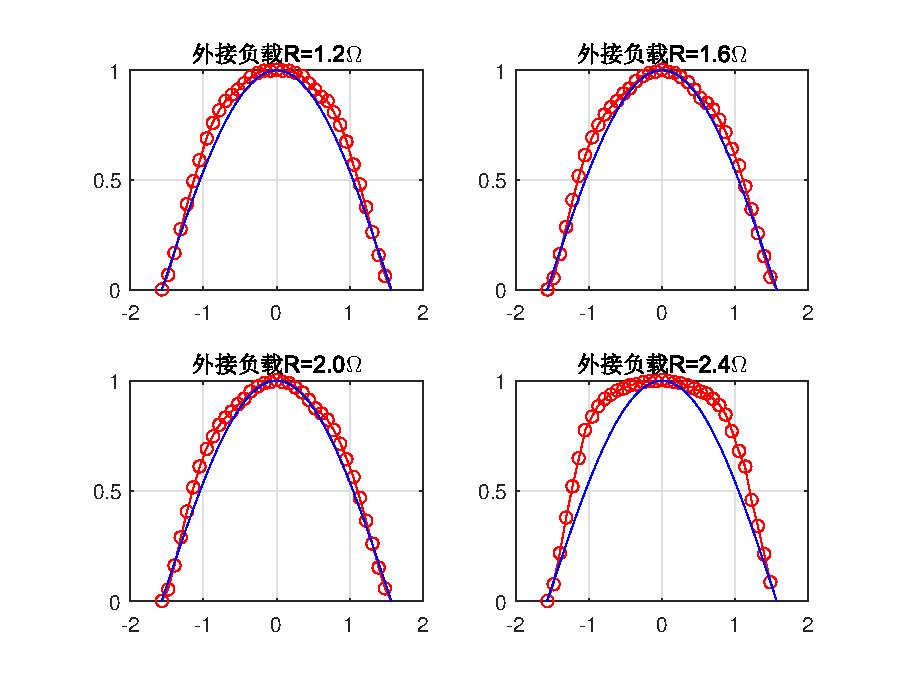
\includegraphics[width=0.65\textwidth]{figure//fig_calculate}
  \caption{SampleFigure1}\label{samplefigure1}
\end{figure}
\end{lstlisting}
\vspace{-0.5ex}

图\ref{samplefigure1} 为以上程序得到图片效果。

若要在页面中并列放置两或者更多张图片,请使用\fbox{$\setminus$begin\{minipage\}}环境,并且使最左侧和最右侧的图片尽量与文字的边缘对齐。考虑到对称性,图片可能需要裁剪来去除部分边缘,通过设置trim属性可以进行裁剪,其四个值按照顺序分别为左侧、下侧、右侧和上侧的裁减量。效果如图\ref{samplefigure2} 和\ref{samplefigure3} 所示。
\newpage
\vspace{-4ex}
\begin{lstlisting}
\begin{figure}[htb]
	\begin{minipage}[b]{0.5\textwidth}
		\flushleft
		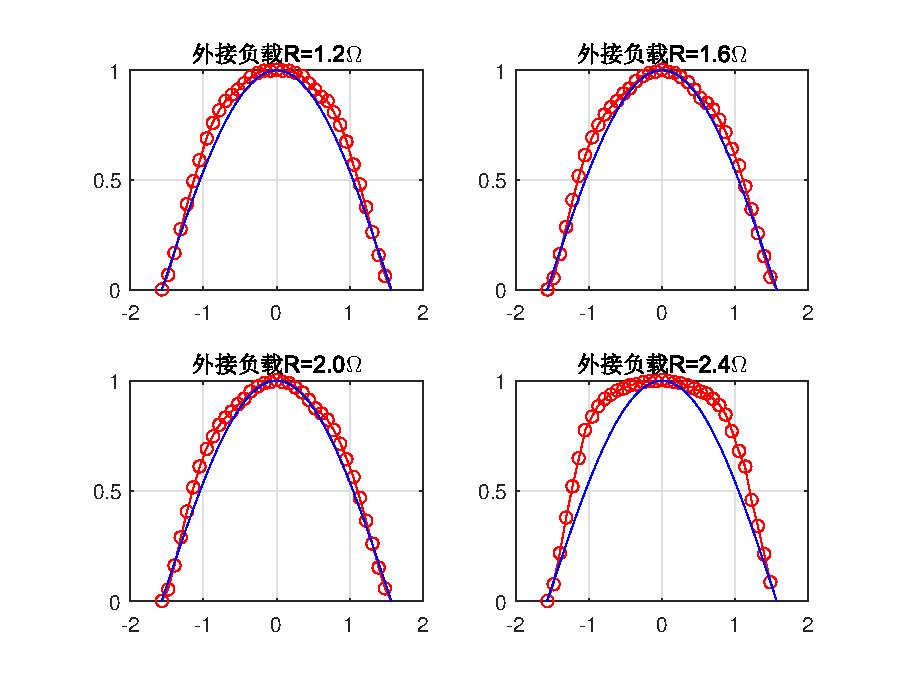
\includegraphics[width=\textwidth,trim=0 20 0 0,clip]{figure//fig_calculate}
		\caption{SampleFigure2}\label{samplefigure2}
	\end{minipage}
	\hfill
	\begin{minipage}[b]{0.5\textwidth}
		\flushright
		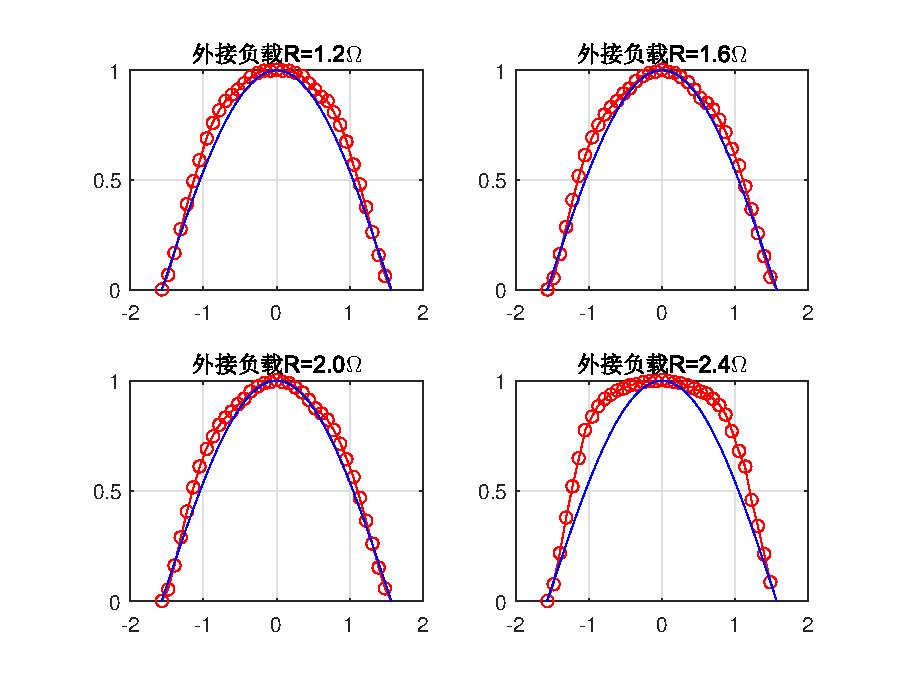
\includegraphics[width=\textwidth,trim=0 20 0 0,clip]{figure//fig_calculate}
		\caption{SampleFigure3}\label{samplefigure3}
	\end{minipage}
\end{figure}
\end{lstlisting}
\vspace{1ex}

\begin{figure}[htbp]
	\centering
	% Requires \usepackage{graphicx}
	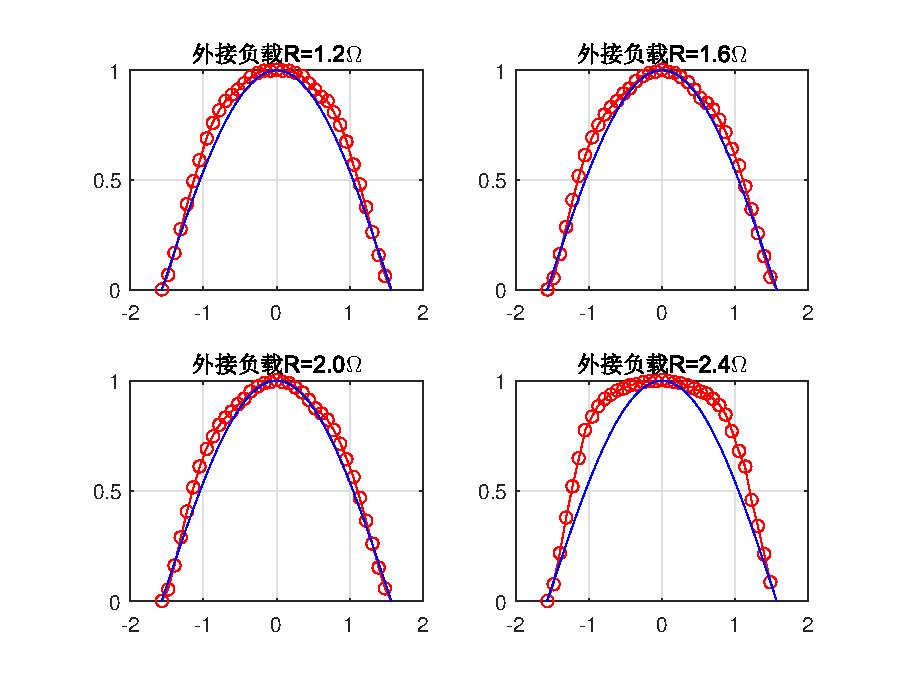
\includegraphics[width=0.6\textwidth, trim=0 20 0 0,clip]{figure//fig_calculate}
	\caption{SampleFigure1}\label{samplefigure1}
\end{figure}

\begin{figure}[htb]
	\begin{minipage}[b]{0.5\textwidth}
		\flushleft
		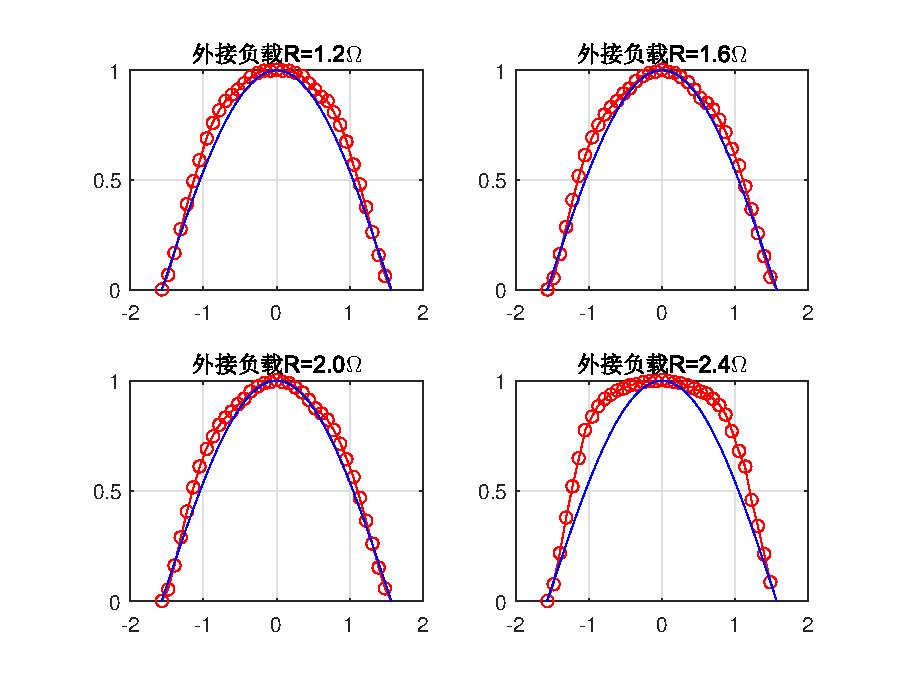
\includegraphics[width=\textwidth,trim=35 20 20 0,clip]{figure//fig_calculate}
		\caption{SampleFigure2}\label{samplefigure2}
	\end{minipage}
	\hfill
	\begin{minipage}[b]{0.5\textwidth}
		\flushright
		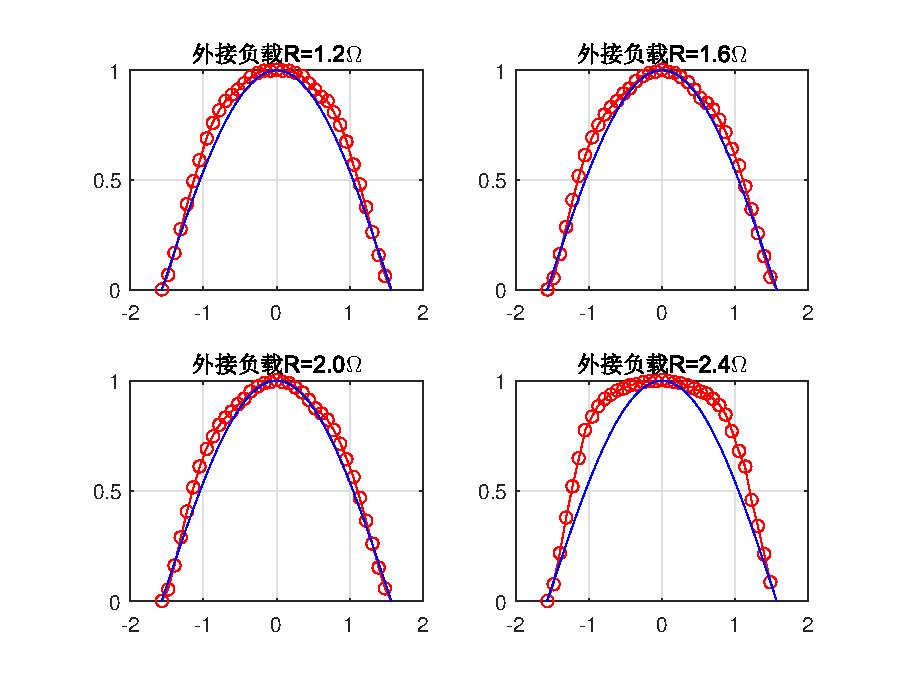
\includegraphics[width=\textwidth,trim=20 20 35 0,clip]{figure//fig_calculate}
		\caption{SampleFigure3}\label{samplefigure3}
	\end{minipage}
\end{figure}

\newpage
\section{表格使用}
由于学校要求三线表格,自己在制作时需要注意该点,表格中的文字应该为五号宋体,结合两点要求,文本框中给出一个表格的范例。为了区分和图片的标题命名,在使用表格时使用“$\setminus$topcaption”,表格标题的格式和前后间距都已经设置。

\vspace{-4ex}
\begin{lstlisting}
{\zihao{5}\songti
\begin{table}[htb]
\begin{center}
\topcaption{SampleTable}\label{sampeltable}
\begin{tabular}{m{3cm} m{2cm} m{2cm} m{2cm}}
  \hline
  Project & A & B & C\\
  \hline
  ProjectOne   & a1 & b1 & c1 \\
  ProjectTwo   & a2 & b2 & c2 \\
  ProjectThree & a3 & b3 & c3 \\
  ProjectFour  & a4 & b4 & c4 \\
  ProjectFive  & a5 & b5 & c5 \\
  \hline
\end{tabular}
\end{center}
\end{table}}
\end{lstlisting}
\vspace{-2ex}

下表\ref{sampeltable}是一个表格示例。

{\wuhao\songti
\begin{table}[htb]
\begin{center}
\topcaption{SampleTable}\label{sampeltable}
\begin{tabular}{m{3cm} m{2cm} m{2cm} m{2cm}}
  \hline
  Project & A & B & C\\
  \hline
  ProjectOne& a1 & b1 & c1 \\
  ProjectTwo & a2 & b2 & c2 \\
  ProjectThree & a3 & b3 & c3 \\
  ProjectFour& a4 & b4 & c4 \\
  ProjectFive & a5& b5 & c5 \\
  \hline
\end{tabular}
\end{center}
\end{table}}

考虑到使用该模板大部分是和我一样的小白,这里做一个小提示,毕业设计由于图表都比较多,如果在正文中用到图1.1、表1.1、 式1.1 等词,最好在正文使用\fbox{图$\setminus$ref\{samplefigure\}}、\fbox{表$\setminus$ref\{sampeltable\}}对图表的标号确定。前提是figure和table已经用\fbox{$\setminus$label\{samplefigure\}}、\fbox{$\setminus$label\{sampeltable\}} 进行标记。每个图标和公式的标记应该是唯一的,重复会出现警告。

上述方法是为了避免在写作过程,突然需要前面的图表和公式进行增添或删减,不再需要手动改图标的标号。

\section{公式使用}
对于公式使用\fbox{$\setminus$begin\{equation\}}环境,如果有多行公式可以使用\fbox{$\setminus$begin\{split\}}环境,符号“\&”为各行公式对齐的位置。

公式和上下文之间默认间距较大,可使用\fbox{$\setminus$equationskip}和\fbox{$\setminus$equationskipfrac}命令来缩小间距,前者适用于简单的单行公式,后者适用于带有分式、矩阵的单行公式或者多行公式。

如果需要对公式中的字母进行注释,并且注释较多,这里推荐一种方法,可以使用表格的环境,表格为2列,第一列字母靠右,第二列解释靠左,如\fbox{$\setminus$begin\{tabular\}\{r@\{---\}l\}}。 
下面文本框中给出了一个多行公式以及注释的示例。

\vspace{-4ex}
\begin{lstlisting}
\begin{equation}\label{SampleEquation}
  \equationskipfrac
  \begin{split}
  \bm{x_}k&=\bm{\Phi}_{k,k-1}\bm{x}_{k-1}+\bm{\Gamma}_{k-1}\bm{w}_{k-1}\\
  \bm{z}_k&=\bm{H}_k\bm{x}_k+\bm{v}_k
  \end{split}
\end{equation}
\begin{tabular}{r@{---}l}
  $\bm{x}_k$  & The state variable of the $k^{th}$ step;\\
  $\bm{z}_k$  & The observation of the $k^{th}$ step; \\
  $\bm{\Phi}_{k,k-1}$ & The transition matrix of the $(k-1)^{th}$ to $k^{th}$ step; \\
  $\bm{\Gamma}_{k-1}$  & The measurement noise driving matrix of the $k^{th}$ step; \\
  $\bm{v}_k$ & The measurement noise of the $k^{th}$ step,$\bm{v_k}\sim N(0,\bm{R}_k)$.
\end{tabular}
\end{lstlisting}
\vspace{-1ex}

下式\ref{sampeltable}和注释为上面程序的效果,数学符号可以自行百度,或者在这\url{http://www.mohu.org/info/symbols/symbols.htm}上面寻找,几乎包含了基本上要用的数学符号。
\begin{equation}\label{SampleEquation}
  \equationskipfrac
  \begin{split}
  \bm{x_}k&=\bm{\Phi}_{k,k-1}\bm{x}_{k-1}+\bm{\Gamma}_{k-1}\bm{w}_{k-1}\\
  \bm{z}_k&=\bm{H}_k\bm{x}_k+\bm{v}_k
  \end{split}
\end{equation}
式中:

\begin{tabular}{r@{---}l}
  $\bm{x}_k$  & The state variable of the $k^{th}$ step;\\
  $\bm{z}_k$  & The observation of the $k^{th}$ step; \\
  $\bm{\Phi}_{k,k-1}$ & The transition matrix of the $(k-1)^{th}$ to $k^{th}$ step; \\
  $\bm{\Gamma}_{k-1}$  & The measurement noise driving matrix of the $k^{th}$ step; \\
  %$\bm{H}_k$  & The measurement matrix of the $k^{th}$ step;\\
  %$\bm{w}_{k-1}$ & The systematic noise of the $(k-1)^{th}$ step ,$\bm{w}_{k-1}\sim N(0,\bm{Q}_{k-1})$;\\
  $\bm{v}_k$ & The measurement noise of the $k^{th}$ step,$\bm{v_k}\sim N(0,\bm{R}_k)$.
\end{tabular}

\newpage
\section{枚举格式}
官方模板未对枚举格式做出规定。但为了方便使用,本模板参考了大部分中文期刊的排版,对枚举格式做出了设置。枚举使用\fbox{$\setminus$begin\{enumerate\}}环境,编号为带有括号的数字,每个item的首行开头缩进两个字符,其余行不缩进。考虑到美观,不建议在item内部进行分段。示例如下:

\vspace{-4ex}
\begin{lstlisting}
\begin{enumerate}
	\item 内容一,内容一,内容一,内容一……
	\item 内容二,内容二,内容二,内容二……
	\item 内容三,内容三,内容三,内容三……
\end{enumerate}
\end{lstlisting}
\vspace{-1ex}

\begin{enumerate}
	\item 内容一,内容一,内容一,内容一,内容一,内容一,内容一,内容一,内容一,内容一,内容一,内容一,内容一。
	\item 内容二,内容二,内容二,内容二,内容二,内容二,内容二,内容二,内容二,内容二,内容二,内容二,内容二。
	\item 内容三,内容三,内容三,内容三,内容三,内容三,内容三,内容三,内容三,内容三,内容三,内容三,内容三。
\end{enumerate}

\section{参考文献}
参考文献在ThesisReference中\fbox{$\setminus$begin\{thebibliography\}}环境中进行填写,具体格式规范查阅参考文献标注国家标准GB/T~7714——2015。按照官方模板的要求,编号和参考文献内容分别左对齐。本模板使用box对编号的位置进行约束\fbox{$\setminus$makebox[1.5em][l]\{[\#1]\}},设定宽度为1.5em,该值适用于一位和两位的编号,若编号达到三位数,则需要自行调整宽度。

模板参考文献使用下面文本框中方法,该方法比较业余,不便于大量参考文献的管理,并且需要手动输入书目信息。专业的方法是使用BibTeX,使用方法自行百度,BibTeX可以在Google scholar、百度学术上直接导入。

\vspace{-4ex}
\begin{lstlisting}
\begin{thebibliography}
\bibitem author,article, year, vol,
\end{thebibliography}
\end{lstlisting}

正文需要引用文献,使用\fbox{$\setminus$cite\{\}}即可。

\section{代码插入}
考虑到大多数同学的代码应该是MATLAB,在ThesisAppendix文件中将语言设置m语言,可以根据自身需要进行改变。网上的Mcode包编译效果非常不错,这里就直接拿来,做一回拿来主义。

Mcode包效果在附录B MATLAB Code中看到,其能较好地还原MATLAB本身的编程风格。程序代码需放到\fbox{$\setminus$begin\{lstlisting\}}环境中。

由于某些未知的原因,如果\fbox{$\setminus$begin\{lstlisting\}}环境跨页,可能会导致页眉出现乱码,所以使用时请注意代码的长度和放置的位置。

建议在\fbox{$\setminus$begin\{lstlisting\}}环境开始前用\fbox{$\setminus$vspace\{-4ex\}},结束后用\fbox{$\setminus$vspace\{-1.5ex\}}来减少代码和上下文之间的距离,具体数值需要按照实际情况调整。

\end{spacing}
}

%-------------------------------------------------------------------------------
%	                        重新制定chapter标题
%-------------------------------------------------------------------------------
\CTEXsetup[titleformat={\heiti\zihao{-3}\centering}]{chapter}%章标题格式
\CTEXsetup[beforeskip={8.0ex}]{chapter}
\CTEXsetup[afterskip={4.5ex}]{chapter}

\chapter*{结\quad 论}
\addcontentsline{toc}{chapter}{结论}

\songti\xiaosi
\begin{spacing}{1.5}

西文字符使用Times New Roman,Happy TeXing!!!

\end{spacing}

\chapter*{致\quad 谢}
\addcontentsline{toc}{chapter}{致谢}

\songti\xiaosi
\begin{spacing}{1.5}

在此论文“NjustThesis Template for Bachelor of Economics , Management \& Arts”模板完成之际,在此向多年来给予我关心和帮助的老师、学长、同学、朋友和家长表示由衷的感谢!

这里需要感谢制作\CTeX 各种宏包的众多前辈的辛勤的付出,没有他们是无法完成这个本科毕设论文模板制作的。

$\dots$


Finally,Happy TeXing!!!

\end{spacing}

\addcontentsline{toc}{chapter}{参考文献}

\setlength{\baselineskip}{18pt}
\songti\xiaosi
\begin{thebibliography}{99}

\bibitem{Leslie.{1994}}
Leslie Lamport. LATEX: A Document Preparation System.AddisonWesley, Reading, Massachusetts, second edition, 1994, ISBN 0-201-52983-1.

\bibitem{Donald.{1984}}
Donald E. Knuth. The TEXbook, Volume A of Computers and Typesetting,Addison Wesley, Reading, Massachusetts, second edition, 1984,ISBN 0-201-13448-9.


\end{thebibliography}

\CTEXsetup[number={\arabic{chapter}}]{chapter}
\CTEXsetup[name={,}]{chapter}
\CTEXsetup[nameformat={\bf\heiti\xiaosan\raggedright}]{chapter}   %	Chapter章节标号格式
\CTEXsetup[titleformat={\bf\heiti\xiaosan\raggedright}]{chapter}      %	Chapter章节标题格式
\CTEXsetup[beforeskip={-8ex}]{chapter}                          
\CTEXsetup[afterskip={1ex}]{chapter}


\lstset{language=Matlab}

\appendix
\begin{appendix}
\chapter{证明}
\begin{spacing}{1.5}
%-------------------------------------------------------------------------------
%	AppendixOne正文部分
%-------------------------------------------------------------------------------
提供一个证明环境,给出一个证明示例。

下面证明命题,如果$\bm{A}$是正交矩阵,那么其特征值为$\pm1$。
\begin{proof}
设$\lambda$ 为正交矩阵的特征值,$\bm{e}$是$\bm{A}$ 属于$\lambda$ 的特征向量,即有:$\bm{A}\bm{e}=\lambda\bm{e}$,且$\bm{e}\neq0$。

上式两边取转置,$\bm{e}^{T}\bm{A}^{T}=\lambda\bm{e}^{T}$。

\text{将}上面两式相乘, $\bm{e}^{T}\bm{A}^{T}\bm{A}\bm{e}=\lambda^2\bm{e}^{T}\bm{e}$。

$\because\bm{A}$是正交矩阵

$\therefore\bm{A}^{T}\bm{A}=\bm{I}$

$\therefore\bm{e}^{T}\bm{e}=\lambda^2\bm{e}^{T}\bm{e}$

又 $\because\bm{e}\neq0$

$\therefore\bm{e}^{T}\bm{e}$ 是一个非零的数

$\therefore\lambda^2=1\Rightarrow\lambda=\pm1$
\end{proof}



\end{spacing}
%------------------------------------------------------------------------------


\chapter{MATLAB Code}
\begin{spacing}{1.5}
%-------------------------------------------------------------------------------
%	AppendixOne正文部分
%-------------------------------------------------------------------------------
下面是一个MATLAB程序的事例,使用了Package mcode,它能较好还原MATLAB本身的编写风格。

\vspace{-4ex}
\begin{lstlisting}
%   The program normalizes the measurement data and compares it to the standard cosine function
data=xlsread('data_sun',1,'B3:E39');
min=[(data(1,1)+data(37,1))/2,(data(1,2)+data(37,2))/2,...
    (data(1,3)+data(37,3))/2,(data(1,4)+data(37,4))/2];
max=[data(19,1),data(19,2),data(19,3),data(19,4)];
Min=repmat(min,37,1);
Max=repmat(max,37,1);
data=(data-Min)./(Max-Min);
x=-pi/2:pi/36:pi/2;
y=cos(x);
%----------------------figure-------------------------%
figure(1);
subplot(2,2,1);
plot(x,data(:,1),'ro-');
hold on;
plot(x,y,'b-');
title('R=1.2\Omega');
axis([-2,2,0,1]);
grid on;
subplot(2,2,2);
plot(x,data(:,2),'ro-');
hold on;
plot(x,y,'b-');
title('R=1.6\Omega');
axis([-2,2,0,1]);
grid on;
subplot(2,2,3);
plot(x,data(:,2),'ro-');
hold on;
plot(x,y,'b-');
title('R=2.0\Omega');
axis([-2,2,0,1]);
grid on;
\end{lstlisting}
\end{spacing}
%------------------------------------------------------------------------------

\end{appendix}


\end{document}
